\chapter{Estadistica, probabilidad e inferencia}

\begin{theorybox}{Sentido estocastico en Matematicas I}
Este capitulo desarrolla el sentido estocastico de Matematicas I: organizacion y analisis de
datos bidimensionales, regresion lineal y cuadratica, correlacion, experimentos aleatorios,
algebra de sucesos, tecnicas de recuento, probabilidad condicionada, probabilidad total,
Bayes e inferencia con herramientas tecnologicas.
\end{theorybox}

\begin{methodbox}{Ruta de estudio}
\begin{enumerate}
  \item Empieza por organizar datos y distinguir poblacion, muestra y variable.
  \item Aprende a leer la nube de puntos antes de calcular una recta de regresion.
  \item Interpreta correlacion y coeficiente de determinacion sin confundirlos con causalidad.
  \item Modeliza el azar mediante espacios muestrales, sucesos y frecuencias relativas.
  \item Cierra con recuento, probabilidad condicionada, arboles, probabilidad total y Bayes.
\end{enumerate}
\end{methodbox}

\section{[C10.S01] Datos bidimensionales y tablas de contingencia}

\subsection*{Objetivos de aprendizaje}
\begin{itemize}
  \item Organizar pares de datos y distribuciones conjuntas.
  \item Obtener distribuciones marginales y condicionadas.
  \item Detectar dependencia estadistica sin confundirla con causalidad.
\end{itemize}

\subsection*{Prerrequisitos}
\begin{itemize}
  \item Porcentajes, frecuencias absolutas y relativas.
\end{itemize}

\begin{theorybox}{Idea minima}
Una variable bidimensional asigna a cada individuo un par \((x_i,y_i)\). Si las variables son
categoricas, una tabla de contingencia recoge las frecuencias conjuntas. Los totales de filas y
columnas son las distribuciones marginales. Una distribucion condicionada se calcula dentro de
un grupo concreto; por ejemplo,
\[
P(B\mid A)=\frac{n(A\cap B)}{n(A)}.
\]
\end{theorybox}

\begin{methodbox}{Como leer una tabla sin mezclar denominadores}
\begin{enumerate}
  \item Identifica si te piden una frecuencia conjunta, marginal o condicionada.
  \item Marca primero el conjunto que actua como condicion.
  \item Divide por el total de ese conjunto, no por el total general.
  \item Compara porcentajes condicionados para estudiar dependencia.
\end{enumerate}
\end{methodbox}

\begin{solvedexample}{[EX-C10.S01-01] Uso de una plataforma de estudio}
En una clase se registra si el alumnado usa una plataforma de practica y si supera una prueba:
\begin{center}
\begin{tabular}{lrrr}
Grupo & Supera & No supera & Total \\
Usa plataforma & 18 & 6 & 24 \\
No la usa & 8 & 8 & 16 \\
Total & 26 & 14 & 40
\end{tabular}
\end{center}
La proporcion que supera la prueba entre quienes usan la plataforma es
\[
P(S\mid U)=\frac{18}{24}=0.75.
\]
Entre quienes no la usan es
\[
P(S\mid \overline U)=\frac{8}{16}=0.50.
\]
Los porcentajes son distintos, por lo que los datos muestran asociacion. No permiten afirmar por
si solos que la plataforma sea la causa de la mejora.
\end{solvedexample}

\begin{commonerror}{Dividir siempre por el total general}
En una probabilidad condicionada el denominador es el total del grupo condicionado. Para
\(P(S\mid U)\), el denominador es \(24\), no \(40\).
\end{commonerror}

\begin{guidedexercise}{[GX-C10.S01-01] Lectura condicionada}
Con la tabla anterior, calcula \(P(U\mid S)\).
\textbf{Pista 1.} Restringe el recuento a quienes superan la prueba.
\end{guidedexercise}
\begin{shortanswer}{[GX-C10.S01-01]} \(P(U\mid S)=\dfrac{18}{26}=\dfrac9{13}\). \end{shortanswer}
\begin{fullsolution}{[GX-C10.S01-01]}
Entre las \(26\) personas que superan la prueba, \(18\) usan la plataforma. Por tanto,
\(P(U\mid S)=18/26=9/13\).
\end{fullsolution}

\subsection*{Practica autonoma graduada}
\begin{exercise}{[PX-C10.S01-01] Calcula la frecuencia relativa conjunta de usar la plataforma y superar la prueba.}\end{exercise}
\begin{exercise}{[PX-C10.S01-02] Calcula la distribucion marginal de superar y no superar.}\end{exercise}
\begin{exercise}{[PX-C10.S01-03] Explica por que la tabla no demuestra causalidad.}\end{exercise}
\begin{shortanswer}{C10.S01 practica autonoma}
\begin{enumerate}
  \item \(18/40=0.45\).
  \item Supera: \(26/40=0.65\); no supera: \(14/40=0.35\).
  \item Es un estudio observacional y pueden existir variables de confusion.
\end{enumerate}
\end{shortanswer}
\begin{fullsolution}{C10.S01 practica autonoma}
\begin{enumerate}
  \item La celda conjunta contiene \(18\) estudiantes y el total es \(40\), luego
  \(P(U\cap S)=18/40=0.45\).
  \item Los totales de columna son \(26\) y \(14\). Al dividir por \(40\), se obtiene
  \(P(S)=26/40=0.65\) y \(P(\overline S)=14/40=0.35\); suman \(1\).
  \item La diferencia entre porcentajes describe asociacion, pero no controla motivacion,
  tiempo de estudio u otras variables de confusion. Por eso no demuestra causalidad.
\end{enumerate}
\end{fullsolution}

\section{[C10.S02] Nubes de puntos, correlacion y causalidad}

\subsection*{Objetivos de aprendizaje}
\begin{itemize}
  \item Interpretar forma, direccion e intensidad de una nube de puntos.
  \item Usar el coeficiente de correlacion lineal \(r\).
  \item Distinguir correlacion, causalidad y correlacion espuria.
\end{itemize}

\subsection*{Prerrequisitos}
\begin{itemize}
  \item Coordenadas cartesianas, media y desviacion tipica.
\end{itemize}

\begin{theorybox}{Idea minima}
El diagrama de dispersion representa cada observacion como un punto \((x_i,y_i)\). El coeficiente
de correlacion lineal cumple \(-1\le r\le 1\). Su signo indica la direccion y \(|r|\) mide la
intensidad de la relacion lineal. Un valor cercano a cero no descarta una relacion no lineal.
\end{theorybox}

\begin{methodbox}{Lectura en cuatro preguntas}
\begin{enumerate}
  \item ¿La nube sube, baja o no muestra direccion clara?
  \item ¿Los puntos siguen aproximadamente una recta o una curva?
  \item ¿Hay valores atipicos que cambien mucho el resultado?
  \item ¿El contexto permite hablar de causa o solo de asociacion?
\end{enumerate}
\end{methodbox}

\begin{solvedexample}{[EX-C10.S02-01] Temperatura y consumo electrico}
Una nube de puntos relaciona temperatura exterior y consumo de aire acondicionado. Se obtiene
\(r=0.91\). Existe una asociacion lineal positiva fuerte: en los datos, las temperaturas altas
tienden a coincidir con consumos altos. El valor \(0.91\) no significa que el \(91\%\) del consumo
este causado por la temperatura ni que todos los puntos esten sobre una recta.
\end{solvedexample}

\begin{commonerror}{Interpretar \(r\) como porcentaje explicado}
El porcentaje de variabilidad explicado por un modelo lineal se relaciona con \(R^2\), no con
\(r\). Ademas, ni \(r\) ni \(R^2\) demuestran causalidad.
\end{commonerror}

\begin{guidedexercise}{[GX-C10.S02-01] Relacion no lineal}
Los puntos siguen aproximadamente una U y se obtiene \(r=0.03\). ¿Puede existir relacion?
\end{guidedexercise}
\begin{shortanswer}{[GX-C10.S02-01]} Si; \(r\) solo mide relacion lineal. \end{shortanswer}
\begin{fullsolution}{[GX-C10.S02-01]}
Las ramas descendente y ascendente pueden compensarse en el calculo de \(r\). La nube muestra
una relacion cuadratica aunque la correlacion lineal sea casi nula.
\end{fullsolution}

\subsection*{Practica autonoma graduada}
\begin{exercise}{[PX-C10.S02-01] Interpreta \(r=-0.82\) en un contexto de velocidad y tiempo de viaje.}\end{exercise}
\begin{exercise}{[PX-C10.S02-02] Decide si \(r=1\) implica causalidad.}\end{exercise}
\begin{exercise}{[PX-C10.S02-03] Explica el efecto posible de un valor atipico sobre \(r\).}\end{exercise}
\begin{shortanswer}{C10.S02 practica autonoma}
\begin{enumerate}
  \item Asociacion lineal negativa fuerte.
  \item No.
  \item Puede aumentar, reducir o incluso cambiar el signo de la correlacion.
\end{enumerate}
\end{shortanswer}
\begin{fullsolution}{C10.S02 practica autonoma}
\begin{enumerate}
  \item Como \(r=-0.82\), el signo indica direccion decreciente y \(|r|=0.82\) indica una
  asociacion lineal fuerte: al aumentar la velocidad, el tiempo tiende a disminuir.
  \item \(r=1\) significa que los datos siguen exactamente una recta creciente, pero no prueba
  un mecanismo causal. Puede existir una causa comun o una relacion construida.
  \item Un valor atipico puede aumentar o reducir \(|r|\), e incluso cambiar su signo. Debe
  revisarse su origen y compararse el calculo con y sin ese punto, sin eliminarlo automaticamente.
\end{enumerate}
\end{fullsolution}

\section{[C10.S03] Regresion lineal y cuadratica}

\subsection*{Objetivos de aprendizaje}
\begin{itemize}
  \item Ajustar e interpretar modelos lineales y cuadraticos.
  \item Usar \(R^2\) y los residuos para valorar un ajuste.
  \item Diferenciar interpolacion y extrapolacion.
\end{itemize}

\subsection*{Prerrequisitos}
\begin{itemize}
  \item Ecuacion de la recta y funciones cuadraticas.
\end{itemize}

\begin{theorybox}{Idea minima}
Una recta de regresion tiene forma \(\hat y=a+bx\). El residuo de un dato es
\(e_i=y_i-\hat y_i\). En un ajuste por minimos cuadrados con termino independiente, el
coeficiente \(R^2\) mide que proporcion de la variabilidad observada de \(y\) recoge el modelo.
Esta medida describe el ajuste en los datos analizados, pero no demuestra causalidad. Un buen
modelo combina ajuste numerico, residuos sin patron y sentido en el contexto.
\end{theorybox}

\begin{methodbox}{Elegir y validar el modelo}
\begin{enumerate}
  \item Representa los datos y decide si la tendencia parece lineal o curvada.
  \item Obtiene el ajuste con calculadora, hoja de calculo o software.
  \item Interpreta los parametros con unidades.
  \item Revisa \(R^2\), los residuos y el intervalo observado antes de predecir.
\end{enumerate}
\end{methodbox}

\begin{solvedexample}{[EX-C10.S03-01] Calibracion de un sensor}
Para entradas \(x=1,2,3,4\), un sensor produce \(y=2.1,4.0,5.9,8.0\). Un ajuste da
\[
\hat y=0.10+1.96x,\qquad R^2=0.999.
\]
Para \(x=2.5\), la prediccion es \(\hat y=0.10+1.96\cdot2.5=5.00\). Es una interpolacion y
resulta fiable dentro de las condiciones medidas. Para \(x=20\) seria una extrapolacion lejana:
el alto \(R^2\) no garantiza que el sensor siga siendo lineal alli.
\end{solvedexample}

\begin{commonerror}{Elegir solo por el mayor \(R^2\)}
Un polinomio complejo puede aumentar \(R^2\) y empeorar la interpretacion o las predicciones.
Hay que valorar la forma de la nube, los residuos, el contexto y la sencillez del modelo.
\end{commonerror}

\begin{guidedexercise}{[GX-C10.S03-01] Interpretar la pendiente}
En \(\hat y=12+0.8x\), donde \(x\) son horas y \(y\) gramos, interpreta \(0.8\).
\end{guidedexercise}
\begin{shortanswer}{[GX-C10.S03-01]} El modelo aumenta \(0.8\) gramos por cada hora adicional. \end{shortanswer}
\begin{fullsolution}{[GX-C10.S03-01]}
La pendiente es la variacion prevista de \(y\) al aumentar \(x\) una unidad. Sus unidades son
gramos por hora.
\end{fullsolution}

\subsection*{Practica autonoma graduada}
\begin{exercise}{[PX-C10.S03-01] Predice \(y\) para \(x=10\) con \(\hat y=3+1.5x\).}\end{exercise}
\begin{exercise}{[PX-C10.S03-02] Calcula el residuo si para \(x=4\) se observa \(y=10\) y el modelo predice \(9.2\).}\end{exercise}
\begin{exercise}{[PX-C10.S03-03] Explica por que no conviene extrapolar muy lejos.}\end{exercise}
\begin{shortanswer}{C10.S03 practica autonoma}
\begin{enumerate}
  \item \(18\).
  \item \(0.8\).
  \item La relacion puede cambiar fuera del intervalo observado.
\end{enumerate}
\end{shortanswer}
\begin{fullsolution}{C10.S03 practica autonoma}
\begin{enumerate}
  \item Se sustituye \(x=10\) en el modelo: \(\hat y=3+1.5\cdot10=18\).
  \item El residuo es observado menos predicho: \(e=y-\hat y=10-9.2=0.8\). Es positivo porque
  el valor observado queda por encima del modelo.
  \item Una extrapolacion lejana supone, sin evidencia, que el patron continua fuera del rango
  observado. Aunque \(R^2\) sea alto, la relacion puede cambiar.
\end{enumerate}
\end{fullsolution}

\section{[C10.S04] Muestreo, inferencia y tecnologia}

\subsection*{Objetivos de aprendizaje}
\begin{itemize}
  \item Distinguir poblacion, muestra, parametro y estadistico.
  \item Reconocer sesgos de seleccion y de respuesta.
  \item Usar una muestra para emitir juicios prudentes.
\end{itemize}

\subsection*{Prerrequisitos}
\begin{itemize}
  \item Proporciones, medias y lectura critica de graficos.
\end{itemize}

\begin{theorybox}{Idea minima}
La poblacion es el conjunto sobre el que se desea concluir; la muestra es el subconjunto
observado. Un estadistico muestral estima un parametro poblacional. Si se mantiene un muestreo
aleatorio comparable, aumentar el tamaño suele reducir la variabilidad muestral, pero no corrige
un procedimiento de seleccion sesgado.
\end{theorybox}

\begin{methodbox}{Auditoria de una conclusion estadistica}
\begin{enumerate}
  \item Identifica poblacion, muestra, variable y forma de seleccion.
  \item Comprueba si algunos grupos han quedado fuera o responden menos.
  \item Revisa unidades, valores ausentes y atipicos con una herramienta digital.
  \item Redacta la conclusion indicando alcance y limitaciones.
\end{enumerate}
\end{methodbox}

\begin{solvedexample}{[EX-C10.S04-01] Encuesta sobre transporte}
Un centro publica una encuesta en la aplicacion que solo usa el alumnado que va en autobus y
concluye que el \(84\%\) de todo el alumnado prefiere ampliar ese servicio. Aunque respondan
muchas personas, la muestra esta autoseleccionada y sobrerrepresenta a quienes usan autobus. La
conclusion no puede generalizarse sin una muestra que incluya de forma adecuada al resto.
\end{solvedexample}

\begin{commonerror}{Creer que una muestra grande siempre es representativa}
Diez mil respuestas obtenidas con un mecanismo sesgado pueden ser menos utiles que una muestra
aleatoria mas pequeña y bien diseñada.
\end{commonerror}

\begin{guidedexercise}{[GX-C10.S04-01] Mejorar el diseño}
Propone una forma de seleccionar una muestra que represente cursos y grupos del centro.
\end{guidedexercise}
\begin{shortanswer}{[GX-C10.S04-01]} Muestreo aleatorio estratificado por curso y grupo. \end{shortanswer}
\begin{fullsolution}{[GX-C10.S04-01]}
Se divide la poblacion por curso y grupo y se selecciona al azar un numero proporcional de
personas en cada estrato. Asi se evita que un unico nivel domine la muestra.
\end{fullsolution}

\subsection*{Practica autonoma graduada}
\begin{exercise}{[PX-C10.S04-01] Identifica poblacion y muestra en una encuesta a 120 de los 900 estudiantes del centro.}\end{exercise}
\begin{exercise}{[PX-C10.S04-02] Explica el sesgo de entrevistar solo a quienes estan en la biblioteca.}\end{exercise}
\begin{exercise}{[PX-C10.S04-03] Redacta una conclusion prudente si 72 de 120 respuestas apoyan una medida.}\end{exercise}
\begin{shortanswer}{C10.S04 practica autonoma}
\begin{enumerate}
  \item Poblacion: 900; muestra: 120.
  \item Excluye a quienes no frecuentan la biblioteca.
  \item En la muestra, el \(60\%\) apoya la medida; la generalizacion depende del muestreo.
\end{enumerate}
\end{shortanswer}
\begin{fullsolution}{C10.S04 practica autonoma}
\begin{enumerate}
  \item La poblacion es el conjunto de \(900\) estudiantes sobre el que se quiere concluir; la
  muestra son las \(120\) personas efectivamente encuestadas.
  \item Entrevistar solo en la biblioteca infrarrepresenta a quienes no la frecuentan. Si el uso
  de la biblioteca se relaciona con la opinion, aparece sesgo de seleccion.
  \item La proporcion muestral es \(72/120=0.60\). La conclusion correcta es: ``el \(60\%\) de
  la muestra apoya la medida''; generalizar a los \(900\) exige justificar el muestreo.
\end{enumerate}
\end{fullsolution}

\section{[C10.S05] Experimentos aleatorios y algebra de sucesos}

\subsection*{Objetivos de aprendizaje}
\begin{itemize}
  \item Construir espacios muestrales y operar con sucesos.
  \item Aplicar complementario, union, interseccion y leyes de Morgan.
  \item Estimar probabilidades mediante frecuencia relativa.
\end{itemize}

\subsection*{Prerrequisitos}
\begin{itemize}
  \item Conjuntos, diagramas de Venn y fracciones.
\end{itemize}

\begin{theorybox}{Idea minima}
El espacio muestral \(\Omega\) contiene los resultados posibles. Los sucesos son subconjuntos de
\(\Omega\). Se cumplen
\[
P(\overline A)=1-P(A),\qquad
P(A\cup B)=P(A)+P(B)-P(A\cap B),
\]
y las leyes de Morgan
\[
\overline{A\cup B}=\overline A\cap\overline B,
\qquad
\overline{A\cap B}=\overline A\cup\overline B.
\]
\end{theorybox}

\begin{methodbox}{Traducir antes de calcular}
\begin{enumerate}
  \item Escribe el experimento y su espacio muestral.
  \item Traduce palabras: ``al menos uno'' suele resolverse con el complementario.
  \item Dibuja un diagrama de Venn si aparecen union e interseccion.
  \item Comprueba que la probabilidad final esta entre \(0\) y \(1\).
\end{enumerate}
\end{methodbox}

\begin{solvedexample}{[EX-C10.S05-01] Control de dos sensores}
Sean \(A\): ``falla el sensor A'' y \(B\): ``falla el sensor B'', con
\(P(A)=0.08\), \(P(B)=0.05\) y \(P(A\cap B)=0.02\). Entonces
\[
P(A\cup B)=0.08+0.05-0.02=0.11.
\]
La probabilidad de que no falle ninguno es el complementario:
\[
P(\overline A\cap\overline B)=1-P(A\cup B)=0.89.
\]
\end{solvedexample}

\begin{commonerror}{Sumar sin restar la interseccion}
Al sumar \(P(A)+P(B)\), los resultados de \(A\cap B\) se cuentan dos veces. Solo puede omitirse
la interseccion cuando los sucesos son incompatibles.
\end{commonerror}

\begin{guidedexercise}{[GX-C10.S05-01] Frecuencia relativa}
En \(500\) simulaciones un suceso ocurre \(137\) veces. Estima su probabilidad.
\end{guidedexercise}
\begin{shortanswer}{[GX-C10.S05-01]} \(137/500=0.274\). \end{shortanswer}
\begin{fullsolution}{[GX-C10.S05-01]}
La frecuencia relativa es \(f_r=137/500=0.274\). Es una estimacion experimental, no una
igualdad exacta que deba repetirse en otra tanda.
\end{fullsolution}

\subsection*{Practica autonoma graduada}
\begin{exercise}{[PX-C10.S05-01] Si \(P(A)=0.37\), calcula \(P(\overline A)\).}\end{exercise}
\begin{exercise}{[PX-C10.S05-02] Si \(P(A)=0.5\), \(P(B)=0.4\) y \(P(A\cap B)=0.2\), calcula \(P(A\cup B)\).}\end{exercise}
\begin{exercise}{[PX-C10.S05-03] Escribe con sucesos ``no ocurre ni A ni B''.}\end{exercise}
\begin{shortanswer}{C10.S05 practica autonoma}
\begin{enumerate}
  \item \(0.63\).
  \item \(0.7\).
  \item \(\overline A\cap\overline B=\overline{A\cup B}\).
\end{enumerate}
\end{shortanswer}
\begin{fullsolution}{C10.S05 practica autonoma}
\begin{enumerate}
  \item Por la regla del complementario,
  \(P(\overline A)=1-P(A)=1-0.37=0.63\).
  \item Se resta la interseccion porque se cuenta dos veces al sumar:
  \(P(A\cup B)=0.5+0.4-0.2=0.7\).
  \item ``No ocurre ni \(A\) ni \(B\)'' significa quedar fuera de ambos sucesos:
  \(\overline A\cap\overline B\). Por Morgan, equivale a \(\overline{A\cup B}\).
\end{enumerate}
\end{fullsolution}

\section{[C10.S06] Regla de Laplace y tecnicas de recuento}

\subsection*{Objetivos de aprendizaje}
\begin{itemize}
  \item Aplicar Laplace solo cuando los resultados elementales son equiprobables.
  \item Usar producto, permutaciones y combinaciones para contar.
  \item Evitar enumeraciones incompletas o con duplicados.
\end{itemize}

\subsection*{Prerrequisitos}
\begin{itemize}
  \item Factoriales y operaciones con fracciones.
\end{itemize}

\begin{theorybox}{Idea minima}
Si los resultados elementales son equiprobables,
\[
P(A)=\frac{\text{casos favorables}}{\text{casos posibles}}.
\]
El principio multiplicativo cuenta procesos por etapas. Si el orden importa aparecen
permutaciones o variaciones; si no importa, combinaciones:
\[
\binom nk=\frac{n!}{k!(n-k)!}.
\]
\end{theorybox}

\begin{methodbox}{Decidir como contar}
\begin{enumerate}
  \item Describe un resultado elemental y comprueba la equiprobabilidad.
  \item Separa el experimento en etapas y multiplica sus opciones.
  \item Pregunta si intercambiar el orden produce un resultado distinto.
  \item Cuenta favorables y posibles con el mismo criterio.
\end{enumerate}
\end{methodbox}

\begin{solvedexample}{[EX-C10.S06-01] Equipo de laboratorio}
De \(8\) estudiantes se eligen \(3\) para formar un equipo, sin cargos. Hay
\[
\binom83=56
\]
equipos. Si dos estudiantes concretos, Ana y Bilal, deben estar juntos, se fija esa pareja y se
elige una persona entre las otras \(6\): hay \(6\) casos favorables. Por tanto,
\[
P(\text{Ana y Bilal juntos})=\frac6{56}=\frac3{28}.
\]
\end{solvedexample}

\begin{commonerror}{Usar combinaciones cuando el orden si importa}
Elegir un equipo de tres personas no es lo mismo que asignar presidencia, secretaria y portavocia.
En el segundo caso los cargos distinguen el orden.
\end{commonerror}

\begin{guidedexercise}{[GX-C10.S06-01] Codigos sin repeticion}
¿Cuantos codigos de tres cifras distintas pueden formarse con \(1,2,3,4,5\)?
\end{guidedexercise}
\begin{shortanswer}{[GX-C10.S06-01]} \(5\cdot4\cdot3=60\). \end{shortanswer}
\begin{fullsolution}{[GX-C10.S06-01]}
Hay \(5\) opciones para la primera posicion, \(4\) para la segunda y \(3\) para la tercera. El
orden importa porque \(123\) y \(321\) son codigos distintos.
\end{fullsolution}

\subsection*{Practica autonoma graduada}
\begin{exercise}{[PX-C10.S06-01] Calcula \(\binom{10}{2}\).}\end{exercise}
\begin{exercise}{[PX-C10.S06-02] Cuenta las ordenaciones de cuatro libros distintos.}\end{exercise}
\begin{exercise}{[PX-C10.S06-03] Al lanzar dos dados, calcula la probabilidad de suma \(7\).}\end{exercise}
\begin{shortanswer}{C10.S06 practica autonoma}
\begin{enumerate}
  \item \(45\).
  \item \(4!=24\).
  \item \(6/36=1/6\).
\end{enumerate}
\end{shortanswer}
\begin{fullsolution}{C10.S06 practica autonoma}
\begin{enumerate}
  \item Como el orden de la pareja no importa,
  \(\binom{10}{2}=10!/(2!8!)=10\cdot9/2=45\).
  \item Para ordenar cuatro libros distintos hay \(4\) opciones para el primero, luego \(3\),
  \(2\) y \(1\): \(4!=4\cdot3\cdot2\cdot1=24\).
  \item Hay \(6\cdot6=36\) resultados equiprobables. Los seis pares que suman \(7\) son
  \[
  (1,6),(2,5),(3,4),(4,3),(5,2),(6,1).
  \]
  Por tanto, \(P=6/36=1/6\).
\end{enumerate}
\end{fullsolution}

\section{[C10.S07] Probabilidad condicionada, total y Bayes}

\subsection*{Objetivos de aprendizaje}
\begin{itemize}
  \item Interpretar probabilidad condicionada e independencia.
  \item Resolver experimentos compuestos con tablas y diagramas de arbol.
  \item Aplicar probabilidad total y Bayes en contexto.
\end{itemize}

\subsection*{Prerrequisitos}
\begin{itemize}
  \item Algebra de sucesos, fracciones y porcentajes.
\end{itemize}

\begin{theorybox}{Idea minima}
Si \(P(A)>0\),
\[
P(B\mid A)=\frac{P(A\cap B)}{P(A)}.
\]
Los sucesos son independientes si \(P(A\cap B)=P(A)P(B)\). Para una particion \(A_i\),
\[
P(B)=\sum_i P(A_i)P(B\mid A_i),
\qquad
P(A_j\mid B)=\frac{P(A_j)P(B\mid A_j)}{P(B)}.
\]
\end{theorybox}

\begin{methodbox}{Arbol de probabilidades}
\begin{enumerate}
  \item Separa las alternativas iniciales en ramas que sumen \(1\).
  \item Escribe en la segunda etapa probabilidades condicionadas.
  \item Multiplica a lo largo de cada camino.
  \item Suma caminos para la probabilidad total y divide para invertir la condicion con Bayes.
\end{enumerate}
\end{methodbox}

\begin{solvedexample}{[EX-C10.S07-01] Alerta de un sistema}
El \(4\%\) de las piezas presenta un defecto. Un sistema alerta en el \(95\%\) de las defectuosas
y tambien alerta por error en el \(3\%\) de las correctas. La probabilidad total de alerta es
\begin{center}
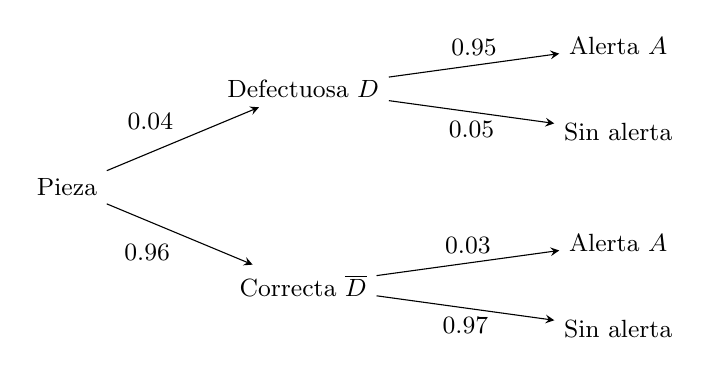
\begin{tikzpicture}[x=1cm,y=1cm,>=stealth,every node/.style={font=\small}]
  \node (o) at (0,0) {Pieza};
  \node (d) at (3,1.25) {Defectuosa \(D\)};
  \node (c) at (3,-1.25) {Correcta \(\overline D\)};
  \node (da) at (7,1.8) {Alerta \(A\)};
  \node (dna) at (7,0.7) {Sin alerta};
  \node (ca) at (7,-0.7) {Alerta \(A\)};
  \node (cna) at (7,-1.8) {Sin alerta};
  \draw[->] (o) -- node[above left] {\(0.04\)} (d);
  \draw[->] (o) -- node[below left] {\(0.96\)} (c);
  \draw[->] (d) -- node[above] {\(0.95\)} (da);
  \draw[->] (d) -- node[below] {\(0.05\)} (dna);
  \draw[->] (c) -- node[above] {\(0.03\)} (ca);
  \draw[->] (c) -- node[below] {\(0.97\)} (cna);
\end{tikzpicture}
\end{center}
\[
P(A)=0.04\cdot0.95+0.96\cdot0.03=0.0668.
\]
Si hay alerta, la probabilidad de defecto es
\[
P(D\mid A)=\frac{0.04\cdot0.95}{0.0668}\approx0.5689.
\]
Una alerta no implica certeza: la baja frecuencia inicial del defecto importa.
\end{solvedexample}

\begin{commonerror}{Intercambiar la condicion}
\(P(A\mid D)\) y \(P(D\mid A)\) responden preguntas distintas. Bayes permite relacionarlas,
pero no pueden intercambiarse sin calcular.
\end{commonerror}

\begin{guidedexercise}{[GX-C10.S07-01] Independencia}
Si \(P(A)=0.4\), \(P(B)=0.5\) y \(P(A\cap B)=0.2\), decide si son independientes.
\end{guidedexercise}
\begin{shortanswer}{[GX-C10.S07-01]} Si, porque \(0.4\cdot0.5=0.2\). \end{shortanswer}
\begin{fullsolution}{[GX-C10.S07-01]}
Se compara la interseccion observada con el producto de probabilidades. Como
\(P(A\cap B)=P(A)P(B)=0.2\), los sucesos son independientes. La positividad solo seria necesaria
si se quisiera expresar la independencia mediante probabilidades condicionadas.
\end{fullsolution}

\subsection*{Practica autonoma graduada}
\begin{exercise}{[PX-C10.S07-01] Si \(P(A\cap B)=0.18\) y \(P(A)=0.6\), calcula \(P(B\mid A)\).}\end{exercise}
\begin{exercise}{[PX-C10.S07-02] Una maquina produce el \(70\%\) de las piezas y otra el \(30\%\); sus tasas de defecto son \(2\%\) y \(5\%\). Calcula la tasa total.}\end{exercise}
\begin{exercise}{[PX-C10.S07-03] Explica por que un positivo no garantiza tener la condicion estudiada.}\end{exercise}
\begin{shortanswer}{C10.S07 practica autonoma}
\begin{enumerate}
  \item \(0.3\).
  \item \(0.7\cdot0.02+0.3\cdot0.05=0.029\).
  \item Depende de falsos positivos y de la frecuencia inicial de la condicion.
\end{enumerate}
\end{shortanswer}
\begin{fullsolution}{C10.S07 practica autonoma}
\begin{enumerate}
  \item La condicion \(A\) fija el denominador:
  \(P(B\mid A)=P(A\cap B)/P(A)=0.18/0.6=0.3\).
  \item La probabilidad total suma los dos caminos de defecto:
  \(0.7\cdot0.02+0.3\cdot0.05=0.014+0.015=0.029\), es decir, \(2.9\%\).
  \item Un positivo puede ser verdadero o falso. Para hallar la probabilidad de tener la
  condicion tras el positivo hay que aplicar Bayes e incorporar su frecuencia inicial o
  prevalencia.
\end{enumerate}
\end{fullsolution}

\begin{challenge}{[CH-C10.S07-01] Auditoria completa de una prediccion}
Diseña una pequeña investigacion con dos variables cuantitativas de tu entorno. Define poblacion y
muestra, recoge al menos \(12\) pares, representa la nube, compara un ajuste lineal y uno
cuadratico, analiza residuos, justifica una prediccion y explica por que no puedes afirmar
causalidad solo con esos datos.
\end{challenge}
\begin{shortanswer}{[CH-C10.S07-01]}
La entrega debe incluir datos, grafico, modelos, \(R^2\), residuos, prediccion y limitaciones.
\end{shortanswer}
\begin{fullsolution}{[CH-C10.S07-01]}
No existe una unica solucion numerica. Se valora que la muestra sea defendible, que los datos y
unidades sean trazables, que el modelo elegido concuerde con la forma de la nube y los residuos,
que la prediccion no extrapole sin justificacion y que la conclusion distinga asociacion de causa.
\end{fullsolution}
